\documentclass[../../../../main.tex]{subfiles}

\begin{document}

\section*{東大理科数学 1964}

\subsection*{第1問}

[解] $a, b, c$ は $t$ の3次方程式
\[
t^3 - z t^2 - y t - x = 0 \quad \cdots \text{①}
\]
の相異なる3解である。したがって、
\[
a^3 + b^3 + c^3 = z(a^2 + b^2 + c^2) + y(a + b + c) + 3x \quad \cdots \text{②}
\]
ここで、
\[
\begin{cases}
bc + ca + ab = -y \\
a + b + c = z
\end{cases}
\]
だから、②に代入して
\[
a^3 + b^3 + c^3 = z(z^2 + 2y) + y z + 3x = z^3 + 3yz + 3x_{\mathbin{/\!/}}
\]

\subsection*{第2問}

[解] $A(t, t^2)$ とする。$AP$ の $m:n$ 内分点は
\[
B\left(\frac{nt+m\alpha}{m+n}, \frac{nt^2+m\beta}{m+n}\right)
\]
で、これが (2) 上にある時、
\[
\frac{nt^2+m\beta}{m+n} = 3\left(\frac{nt+m\alpha}{m+n}\right)^2 + 24\left(\frac{nt+m\alpha}{m+n}\right) + 50 \quad \cdots \text{①}
\]
これが任意の $t \in \mathbb{R}$ で成立するので、①が $t$ についての恒等式である。係数比較して
\[
\begin{cases}
\frac{n}{m+n} = 3\left(\frac{n}{m+n}\right)^2 \\
0 = 6\frac{n m \alpha}{(m+n)^2} + 24\frac{n}{m+n} \\
\frac{m\beta}{m+n} = 3\left(\frac{m\alpha}{m+n}\right)^2 + 24\frac{m\alpha}{m+n} + 50
\end{cases}
\]
\[
\therefore \begin{cases}
m+n = 3n & \cdots \text{②} \\
0 = \frac{m\alpha}{m+n} + 4 \quad (\because n, m > 0) & \cdots \text{③} \\
m\beta = 3\frac{(m\alpha)^2}{m+n} + 24m\alpha + 50(m+n) & \cdots \text{④}
\end{cases}
\]
②から、$m = 2n \quad \cdots$ ⑤だから、③, ④に代入して、
\[
\alpha = -6, \quad \beta = 3_{\mathbin{/\!/}}
\]
又、⑤から $m:n = 2:1_{\mathbin{/\!/}}$

\subsection*{第3問}

[解] 平面 $\text{PBC}$ と辺 $\text{VD}$ の交点を $\text{Q}$ とすると $\text{Q}$ も $\text{VD}$ を $3:1$ に内分する。したがって、
\[
|\text{PQ}| = \frac{3}{4} |\text{AD}| = 15 \, [\text{cm}]
\]
又、$\text{AD}, \text{BC}$ の中点を $\text{M}, \text{N}$ として、$\triangle\text{VMN}$ で立体を切ると右図。ただし、$\text{R}$ は $\text{PQ}$ の中点である。
\[
\cos \angle \text{RMN} = \frac{1}{4}
\]
だから、$\triangle\text{MNR}$ に余弦定理を用いて、
\[
|\text{RN}| = \sqrt{(10)^2 + (20)^2 - 2 \cdot 10 \cdot 20 \cdot \frac{1}{4}} = 20
\]
したがって切り口 (台形 $\text{PQCB}$) の面積は
\[
\frac{1}{2} \cdot (|\text{PQ}| + |\text{BC}|) \cdot |\text{RN}| = \frac{1}{2} (15 + 20) \cdot 20 = 350 \, [\text{cm}^2]_{\mathbin{/\!/}}
\]

\begin{center}
\begin{tikzpicture}[scale=0.85, >=stealth]
  % Pyramid V-ABCD
  \coordinate (V) at (2, 4);
  \coordinate (A) at (0, 0);
  \coordinate (B) at (3, -0.8);
  \coordinate (C) at (4.5, 0.5);
  \coordinate (D) at (1.5, 1.3);
  
  \draw[thick] (V) -- (A);
  \draw[thick] (V) -- (B);
  \draw[thick] (V) -- (C);
  \draw[dashed] (V) -- (D);
  
  \draw[thick] (A) -- (B) node[midway, below] {$20$};
  \draw[thick] (B) -- (C);
  \draw[dashed] (C) -- (D);
  \draw[dashed] (D) -- (A);

  \coordinate (P) at ($(V)!0.75!(A)$);
  \coordinate (Q) at ($(V)!0.75!(D)$);

  \node[left] at (P) {$P$};
  \node[above left] at (Q) {$Q$};

  \fill (P) circle (1.5pt);
  \fill (Q) circle (1.5pt);

  \coordinate (H) at (2, 0.25);
  \draw[dashed] (V) -- (H) node[midway, right] {$40$};

  \node[above] at (V) {$V$};
  \node[below left] at (A) {$A$};
  \node[below right] at (B) {$B$};
  \node[right] at (C) {$C$};
  \node[above left] at (D) {$D$};

  \node[above left] at ($(V)!0.375!(A)$) {\scriptsize \textcircled{3}};
  \node[below left] at ($(P)!0.5!(A)$) {\scriptsize \textcircled{1}};
  \node[above left] at ($(V)!0.375!(D)$) {\scriptsize \textcircled{3}};
\end{tikzpicture}
\quad
\begin{tikzpicture}[scale=0.85, >=stealth]
  \coordinate (V) at (2, 3.5);
  \coordinate (M) at (0, 0);
  \coordinate (N) at (4, 0);
  
  \draw[thick] (M) -- (N) node[midway, below] {$20$};
  \draw[thick] (V) -- (M) node[midway, above left] {$40$};
  \draw[thick] (V) -- (N) node[midway, above right] {$40$};

  \draw[dashed] (V) -- (2, 0);
  \draw (2, 0) -- (2, 0.3) -- (1.7, 0.3);

  \coordinate (R) at ($(V)!0.75!(M)$);
  \fill (R) circle (1.5pt) node[left] {$R$};
  
  \draw[thick] (R) -- (N);

  \node[above] at (V) {$V$};
  \node[below left] at (M) {$M$};
  \node[below right] at (N) {$N$};

  \node[above left] at ($(V)!0.375!(M)$) {\scriptsize \textcircled{3}};
  \node[below left] at ($(R)!0.5!(M)$) {\scriptsize \textcircled{1}};
\end{tikzpicture}
\end{center}

\subsection*{第4問}

[解] $P_k(x_k, y_k)$ とおく。題意から
\[
\begin{pmatrix} x_1 \\ y_1 \end{pmatrix} = \frac{1}{2} \begin{pmatrix} x_4 \\ y_4 \end{pmatrix} + \frac{1}{2} \begin{pmatrix} 0 \\ 2 \end{pmatrix}
\]
\[
\begin{pmatrix} x_2 \\ y_2 \end{pmatrix} = \frac{1}{2} \begin{pmatrix} x_1 \\ y_1 \end{pmatrix} + \frac{1}{2} \begin{pmatrix} 0 \\ 0 \end{pmatrix}
\]
\[
\begin{pmatrix} x_3 \\ y_3 \end{pmatrix} = \frac{1}{2} \begin{pmatrix} x_2 \\ y_2 \end{pmatrix} + \frac{1}{2} \begin{pmatrix} 1 \\ 0 \end{pmatrix}
\]
\[
\begin{pmatrix} x_4 \\ y_4 \end{pmatrix} = \frac{1}{2} \begin{pmatrix} x_3 \\ y_3 \end{pmatrix} + \frac{1}{2} \begin{pmatrix} 2 \\ 2 \end{pmatrix}
\]
これをといて
\[
P_1\left(\frac{2}{3}, \frac{8}{5}\right), \quad P_2\left(\frac{1}{3}, \frac{4}{5}\right), \quad P_3\left(\frac{2}{3}, \frac{2}{5}\right), \quad P_4\left(\frac{4}{3}, \frac{6}{5}\right)_{\mathbin{/\!/}}
\]
となり、右図から、この面積 $S$ は
\[
S = \frac{1}{2} \cdot \left(\frac{8}{5} - \frac{2}{5}\right) \cdot \left(\frac{4}{3} - \frac{1}{3}\right) = \frac{3}{5}_{\mathbin{/\!/}}
\]

\begin{center}
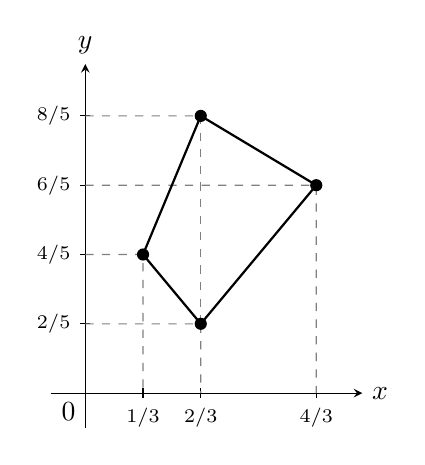
\begin{tikzpicture}[scale=2.2, >=stealth]
  % Axes
  \draw[->] (-0.2, 0) -- (1.6, 0) node[right] {$x$};
  \draw[->] (0, -0.2) -- (0, 1.9) node[above] {$y$};

  \node[below left] at (0,0) {$0$};

  \coordinate (P1) at (2/3, 8/5);
  \coordinate (P2) at (1/3, 4/5);
  \coordinate (P3) at (2/3, 2/5);
  \coordinate (P4) at (4/3, 6/5);

  % Ticks on x-axis
  \draw (1/3, 0.03) -- (1/3, -0.03) node[below] {\scriptsize $1/3$};
  \draw (2/3, 0.03) -- (2/3, -0.03) node[below] {\scriptsize $2/3$};
  \draw (4/3, 0.03) -- (4/3, -0.03) node[below] {\scriptsize $4/3$};

  % Ticks on y-axis
  \draw (0.03, 8/5) -- (-0.03, 8/5) node[left] {\scriptsize $8/5$};
  \draw (0.03, 6/5) -- (-0.03, 6/5) node[left] {\scriptsize $6/5$};
  \draw (0.03, 4/5) -- (-0.03, 4/5) node[left] {\scriptsize $4/5$};
  \draw (0.03, 2/5) -- (-0.03, 2/5) node[left] {\scriptsize $2/5$};

  % Dashed lines
  \draw[dashed, gray] (0, 8/5) -- (P1);
  \draw[dashed, gray] (0, 6/5) -- (P4) -- (4/3, 0);
  \draw[dashed, gray] (0, 4/5) -- (P2) -- (1/3, 0);
  \draw[dashed, gray] (0, 2/5) -- (P3) -- (2/3, 0);
  \draw[dashed, gray] (P1) -- (P3);

  % Polygon
  \draw[thick] (P1) -- (P4) -- (P3) -- (P2) -- cycle;

  % Points
  \fill (P1) circle (1pt);
  \fill (P2) circle (1pt);
  \fill (P3) circle (1pt);
  \fill (P4) circle (1pt);
\end{tikzpicture}
\end{center}

\end{document}
